\chapter[Image Processing]{Image\\ Processing}
\label{chap:image_processing}
\index{image processing|(}

% Position the image to the right of the heading.
\vspace{-9\baselineskip} % move up
\hfill
 \begin{minipage}{0.5\textwidth}
 \centering
 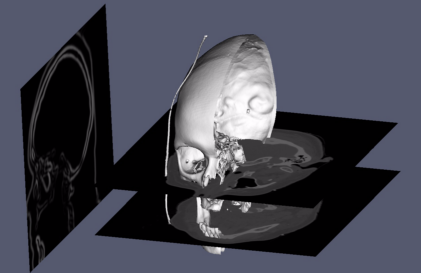
\includegraphics{VTKTextbook-216}
  \captionof*{figure}{\textit{Gradient magnitude of a slice (vertical) of the Visible Woman CT dataset shown with an isosurface and two slices (horizontal) of the dataset.}}
 \end{minipage}
\vspace{2\baselineskip}

\firstletter{I}n this chapter we describe the image processing components of the Visualization Toolkit.
The focus is on key representational ideas, pipeline issues such as data streaming, and useful algorithms for improving the appearance and effectiveness of image data visualizations.

\section{Introduction}

Image processing has been a mainstay of computing since the advent of the digital computer. Early efforts focused on improving image content for human interpretation. More recently image processing has been utilized by practitioners of computer vision, the goal being the processing of image data for autonomous machine perception \cite{Gonzalez92}. From the perspective of data visualization, image processing is used to manipulate image content to improve the results of subsequent processing and interpretation. For example, a CT or MRI scan may generate spurious signal noise or require image segmentation. Using the techniques of image processing, noise can be removed and automatic and semi-automatic segmentation can be performed on a slice by slice (i.e., image by image basis). As a result, isosurface generation, volume rendering, and other 3D techniques can be improved in appearance, accuracy, and effectiveness by applying techniques from image processing.

Since the focus of this text is on 3D graphics and visualization, this chapter treats image processing in a limited way. However, we would like to emphasize the interrelationship of image processing, computer graphics, and visualization. Often texts and courses treat these as distinctly separate disciplines, when in fact they are closely related (see ``Imaging, Computer Graphics, and Visualization''on page \pageref{sec:imaging_computer_graphics_visualization}).

The material presented here was selected to demonstrate a number of important points. First, the data flow or pipeline approach presented earlier is directly applicable to image processing, with the added benefit that we can easily implement data streaming and caching due to the regular nature of image data. Second, image processing algorithms can improve the results of visualization. We will show this through a number of useful examples. And finally, from a practical point of view, we wanted to demonstrate a system architecture that includes imaging, graphics, and visualization.

\section{Data Representation}
\index{data representation!in image processing|(}\index{image processing!data representation|(}

In this section we will briefly describe the data representation behind the imaging pipeline. As we saw earlier (in ``The Dataset'' on page \pageref{sec:dataset}), a dataset consists of both a structure (topology and geometry) and data attributes. Although in principle an image can be represented as a image data dataset, the special nature of image processing suggests a more complex representation, as we will soon see.

An image is typically used to refer to a 2D structured point dataset. More generally, in this chapter we will define an image as consisting of up to four dimensions: three spatial dimensions x, y, and z, and time t. The reason we add the time dimension is that images are frequently generated as a time series, and we often wish to access the data along the time axis. For example, we may plot the value at a point as a function of time.

As described in ``Image Data'' on \pageref{subsec:image_data}), an image has both regular topology and geometry. The regularity of the data lends itself to many special operations. In particular, we can support data caching and \emph{streaming}, and operating on \emph{regions of interest} in the data.

\subsection{Regions of Interest}
\index{region of interest}

When data has a regular spatial organization, it is possible to request the data in pieces or regions of interest. For example, a mapper may need only a region of the data for its display, so loading or processing the whole dataset would be inefficient. An example of this is a two--dimensional viewer that displays only one slice of a large structured volume. By loading slices only as they are needed, disk access can be reduced, and memory conserved.

\begin{figure}[htb]
	\begin{subfigure}[h]{0.36\linewidth}
		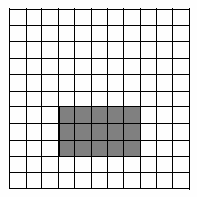
\includegraphics[width=0.96\linewidth]{Figure10-1a}
		\captionsetup{justification=centering}
		\caption*{Axis aligned matrix (rectangular region)}
		\label{fig:Figure10-1a}
	\end{subfigure}
	\hfill
	\begin{subfigure}[h]{0.36\linewidth}
    % Dummy spacer
	\end{subfigure}
	\hfill
	\begin{subfigure}[h]{0.36\linewidth}
		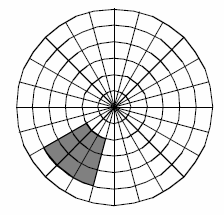
\includegraphics[width=0.96\linewidth]{Figure10-1b}
		\captionsetup{justification=centering}
		\caption*{Polar coordinate grid (pie shaped region)}
		\label{fig:Figure10-1b}
	\end{subfigure}
	\caption{Axis aligned matrices naturally lend themselves to rectangular regions, and polar coordinate grids to pie-shaped regions.}\label{fig:Figure10-1}
\end{figure}

Although regions of interest can have arbitrary shapes, the regular structure of the data samples determines optimal region configurations. An image stored in a Cartesian coordinate system easily divides into smaller rectangular regions, while data sampled on a polar coordinate grid is best divided into pie-shaped regions (Figure \ref{fig:Figure10-1}). Therefore, operating on regions of data means that we process ``windows'' of data specified by $(min,max)$ ranges of each dimension, or axis. For example, a region in a 2D image of dimensions $100 \times 100$ might be specified as $(25,49, 0,49)$, meaning that we would operate on a $(25 \times 50)$ window.
\index{region of interest}

\subsection{Streaming and Caching}

The disadvantage of processing regions of interest is that the same data may be read and processed multiple times. If the viewer described above needs to cine (i.e., loop) through the slices, or interactively pan around a large image, it would be beneficial to have all the data loaded at once.

A compromise between the two extreme approaches of maintaining all data in memory or operating on small pieces is to update regions larger than requested, but not as large as the whole image. This is referred to as a data cache\index{caching}\index{data cache}. Data caching anticipates future requests and works well in most cases. However, it breaks down when there is little or no coherence between subsequent requests.

With the region--processing model, the data objects can be thought of as caches that hold any number of regions. There are numerous caching strategies for saving and releasing regions that can be quite complex. The simplest strategy saves only a single region at any one time. If subsequent requests are completely contained in the cached region, no further processing is required. An alternative strategy might divide an image into tiled regions of all the same size. When a region larger than the tile is requested, multiple tiles are updated to cover the region. When designing a caching strategy, it is important to consider the overhead of copying data to change its format. Some of the advantages of complex strategies are lost when all the factors are considered.

Given the ability to operate on regions of data, it is a small step to \emph{stream} operations on a whole dataset. Streaming\index{streaming} is the process of pulling regions of data in a continual flow through the pipeline. For instance, a pixel histogram mapper could request single pixels as it accumulates values in its bins. Large datasets can be processed in this manner without ever having to load more than a few pixels at a time. If multiple processors are available, region processing can also be used to split a task into multiple pieces for load balancing and faster execution.

\subsection{Attribute Data and Components}

Unlike visualization algorithms that may generate normals, vectors, tensors, and texture coordinates, image processing algorithms generally process attribute data consisting of scalar data. Often the data is a single component (e.g., a gray-scale image), but frequently color images (three components of RGB, for example) may also be processed.

In the \emph{Visualization Toolkit} imaging pipeline, attribute data is represented as n-dimensional component data. Refer to ``Putting It All Together'' on page \pageref{sec:chap10.putting_it_all_together}) to see the implementation details for component data, regions of interest, streaming, and caching.
\index{data representation!in image processing|)}\index{image processing!data representation|)}

\section{Algorithms}
\index{algorithms!image processing|(}\index{image processing algorithms|(}

This section provides an overview and examples for important image processing algorithms. The importance of the algorithms is measured on their relevance to 3D data visualization. Topics include: removing noise, smoothing\index{smoothing}, reducing sampling artifacts, image enhancement, segmentation, and morphological operators such as erosion and dilation.

\subsection{Image Restoration}
\index{image processing algorithms!image restoration|(}\index{image restoration|(}

Noise and other artifacts are inherent in all methods of data acquisition. Since artifacts can degrade the visual appearance and analysis of images, the first step of image processing is often restoration. Knowledge of the statistical properties of artifacts allows filters to selectively remove them with minimal impact on the underlying data. For example, most of the power of typical images lie in low frequencies, while white noise is evenly distributed across the frequency spectrum. In this situation, low-pass filters eliminate much of the noise, but leave most of the image intact.

\begin{figure}[htb]
	\begin{subfigure}[h]{0.24\linewidth}
		
\includegraphics[width=0.96\linewidth]{Figure10-2a}
		\captionsetup{justification=centering}
		\caption*{Gaussian Kernel}
		\label{fig:Figure10-2a}
	\end{subfigure}
	\hfill
	\begin{subfigure}[h]{0.98\linewidth}
		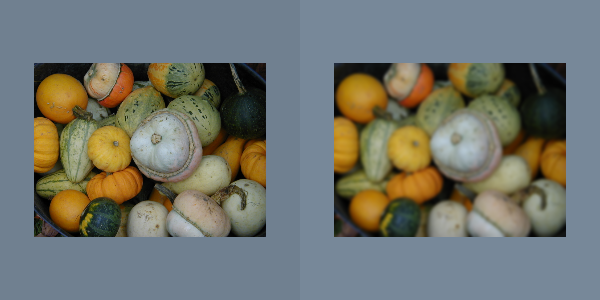
\includegraphics[width=0.96\linewidth]{Figure10-2b}
		\captionsetup{justification=centering}
		\caption*{Original image (left). Convolution (right):
         $f \star k(x,y) = \sum_{ij}f(i,j)k((x-i),(y-j))$\\ (\href{https://lorensen.github.io/VTKExamples/site/Cxx/ImageProcessing/GaussianSmooth/}{GaussianSmooth.cxx} or \href{https://lorensen.github.io/VTKExamples/site/Python/ImageProcessing/GaussianSmooth/}{GaussianSmooth.py})}
		\label{fig:Figure10-2b}
	\end{subfigure}
	\caption{Low-pass filters can be implemented as convolution with a Gaussian kernel. The Gaussian kernel displayed on top has been magnified for this figure.}\label{fig:Figure10-2}
\end{figure}

A simple implementation of a low-pass smoothing filter is convolution\index{convolution} with a kernel with all positive values. The typical kernels used for smoothing are either constant across a circular neighborhood, or have a Gaussian profile (see Figure \ref{fig:Figure10-2}). Gaussian smoothing\index{Gaussian smoothing} results in better looking images than smoothing with constant kernels, but can be more computationally expensive because of the large kernel size necessary to capture the Gaussian profile. Smoothing becomes even more expensive when it is generalized to three--dimensional datasets, and three--dimensional kernels.

One way to speed Gaussian smoothing is to decompose the filter into two 1D convolutions. Since the 2D Gaussian function is separable,

\begin{equation}\label{eq:10.1}
g(i, j) = \dfrac{1}{2\pi \sigma^2} \exp\left(-\dfrac{i^2 + j^2}{2\sigma^2} \right)
        = \dfrac{1}{\sqrt{2\pi}\sigma} \exp\left(-\dfrac{i^2}{2\sigma^2} \right)
          \dfrac{1}{\sqrt{2\pi}\sigma} \exp\left(-\dfrac{j^2}{2\sigma^2} \right)
\end{equation}
\myequations{Decomposing a 2D Gaussian function into two 1D convolutions.}

\noindent smoothing along the \emph{x} axis and then along the \emph{x} axis with 1D Gaussian kernels is equivalent to convolving with a 2D Gaussian kernel. It is also possible to approximate Gaussian smoothing by convolving with a constant binary kernel multiple times.
\index{image processing algorithms!image restoration|)}\index{image restoration|)}

\subsection{Nonlinear Smoothing}
\index{image processing algorithms!non--linear smoothing|(}\index{non--linear smoothing|(}\index{smoothing!non--linear|(}

One problem with simple smoothing to remove noise is that edges are blurred. Although high frequencies make up a small part of images, the human visual system is acutely sensitive to high frequencies in the spatial form of edges. In fact, most of the low frequencies in an image are discarded by the visual system before it even leaves the retina. One approach to smoothing that preserves edges is anisotropic diffusion\index{diffusion anisotropic}. This filter smooths relatively flat regions of an image, but does not diffuse across abrupt transitions. The diffusion is iterated until the desired level of noise reduction is reached. Two possible diffusion criteria are: Diffuse only when the gradient magnitude is below a specified value, or diffuse two pixels only when the difference between the pixels is lower than a specified constant.

\begin{figure}[!htb]
	\centering
	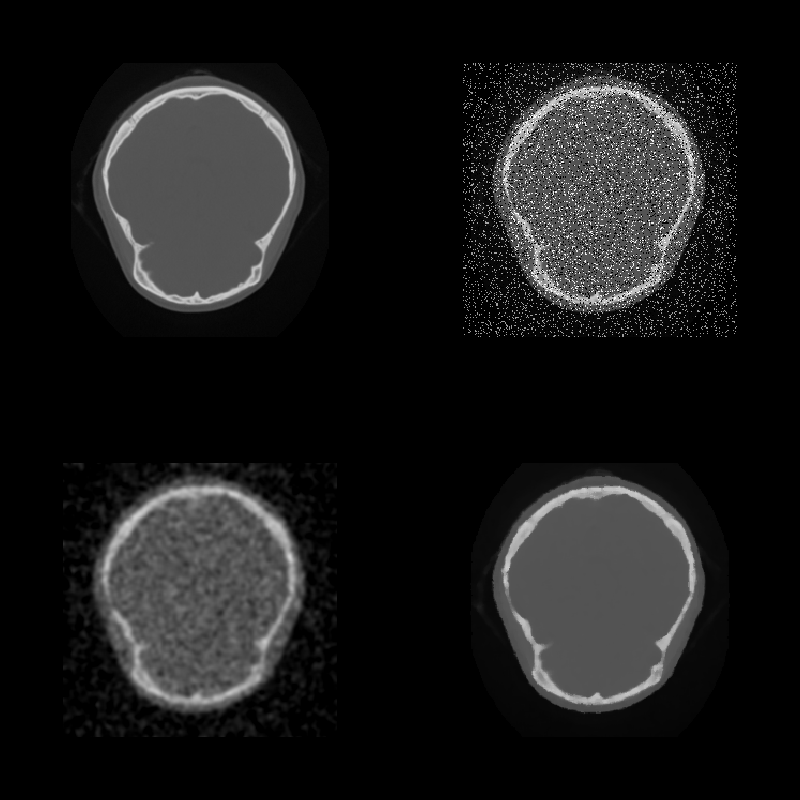
\includegraphics[width=0.98\textwidth]{Figure10-3}
	\caption{Comparison of Gaussian and Median smoothing for reducing low-probability high-amplitude noise. Top row: Original image (left); Noisy image (right). Bottom row: Gaussian smoothing (left); Median smoothing (right). (\href{https://lorensen.github.io/VTKExamples/site/Cxx/ImageProcessing/MedianComparison/}{MedianComparison.cxx} or \href{https://lorensen.github.io/VTKExamples/site/Python/ImageProcessing/MedianComparison/}{MedianComparison.py})}
	\label{fig:Figure10-3}
\end{figure}

\begin{figure}[htb]
	\begin{subfigure}[h]{0.96\linewidth}
		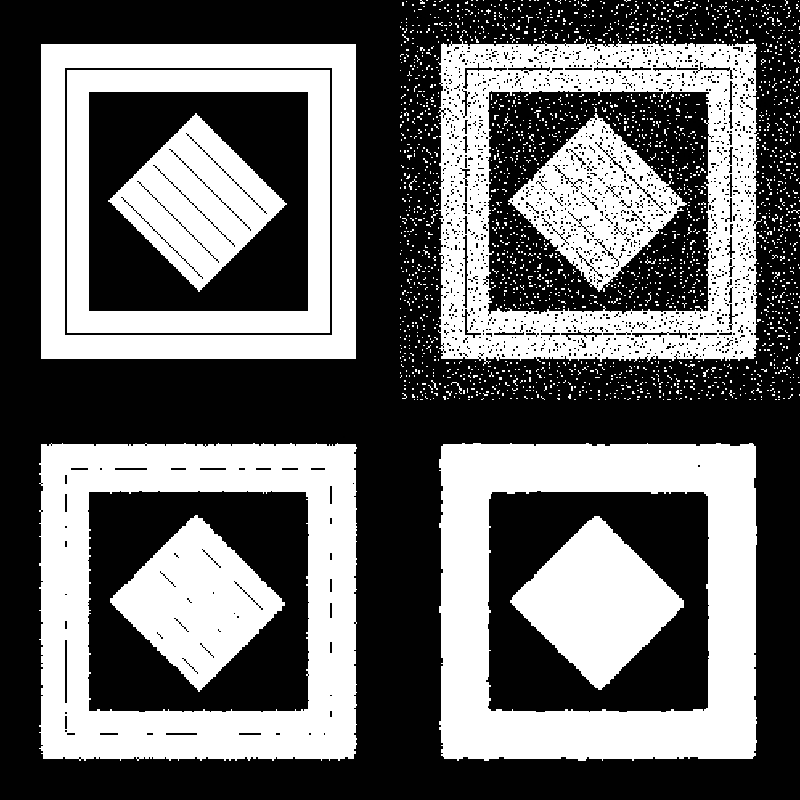
\includegraphics[width=0.96\linewidth]{Figure10-4a}
		\captionsetup{justification=centering}
		\caption*{See: (\href{https://lorensen.github.io/VTKExamples/site/Cxx/ImageProcessing/HybridMedianComparison/}{HybridMedianComparison.cxx} or \href{https://lorensen.github.io/VTKExamples/site/Python/ImageProcessing/HybridMedianComparison/}{HybridMedianComparison.py})}
		\label{fig:Figure10-4a}
	\end{subfigure}
	\hfill
	\begin{subfigure}[h]{0.32\linewidth}
		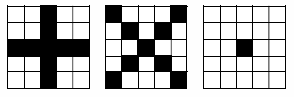
\includegraphics[width=0.96\linewidth]{Figure10-4b}
		\captionsetup{justification=centering}
		\caption*{Hybrid--Median Neighborhoods}
		\label{fig:Figure10-4b}
	\end{subfigure}
	\caption{Comparison of median and hybrid-median filters. The hybrid filter preserves corners and thin lines, better than the median filter. The lower patterns represent the three neighborhoods used to compute the hybrid median. Top row: Original image (left); Noisy image (right). Middle row: Hybrid-median filter (left); Median filter (right).}\label{fig:Figure10-4}
\end{figure}

A median filter\index{median filter} also smooths while preserving edges. This filter replaces each pixel with the median value of the scalar values in a neighborhood centered on the pixel. Median filters are most effective on high amplitude noise that has a low probability of occurring (see Figure \ref{fig:Figure10-3}). There are two ways to control the amount and scale of noise removed: The size of the neighborhood can be varied, or the filter can be applied multiple times. This median filter preserves edges; however, it does round corners and remove thin lines. The hybrid median filter was developed to address this behavior. It operates on a $5 \times 5$ neighborhood around each pixel. The algorithm consists of two steps: first the median values of an ``x''--shaped and ``+''--shaped neighborhoods are computed, then the median of these two values and the center-pixel value is computed to give the final result. The hybrid median has a fixed size neighborhood, but can be applied multiple times to further reduce noise (Figure \ref{fig:Figure10-4}).
\index{image processing algorithms!non--linear smoothing|)}\index{non--linear smoothing|)}\index{smoothing!non--linear|)}

\subsection{Low Frequency Artifacts}
\index{image processing algorithms!low frequency artefacts|(}

\begin{figure}[htb]
	\begin{subfigure}[h]{0.96\linewidth}
		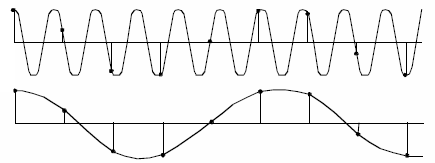
\includegraphics[width=0.96\linewidth]{Figure10-5a}
		\captionsetup{justification=centering}
		\caption*{}
		\label{fig:Figure10-5a}
	\end{subfigure}
	\hfill
	\begin{subfigure}[h]{0.96\linewidth}
		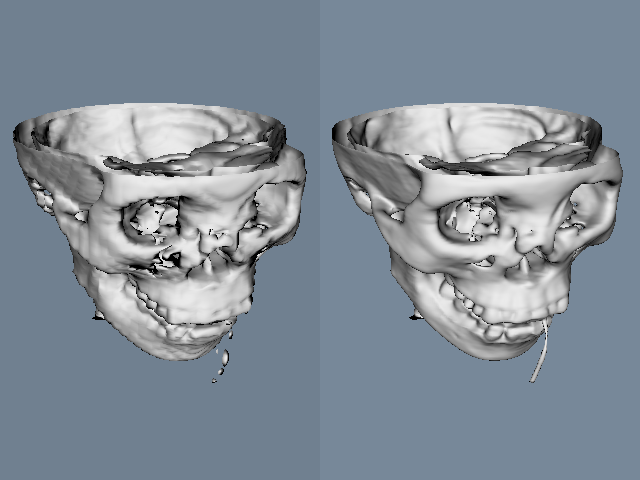
\includegraphics[width=0.96\linewidth]{Figure10-5b}
		\captionsetup{justification=centering}
		\caption*{See: (\href{https://lorensen.github.io/VTKExamples/site/Cxx/ImageProcessing/IsoSubsample/}{IsoSubsample.cxx} or \href{https://lorensen.github.io/VTKExamples/site/Python/ImageProcessing/IsoSubsample/}{IsoSubsample.py})}
		\label{fig:Figure10-5b}
	\end{subfigure}
	\caption{This figure demonstrates aliasing that occurs when a high-frequency signal is subsampled. High frequencies appear as low frequency artifacts. The lower left image is an isosurface of a skull after subsampling. The right image used a low-pass filter before subsampling to reduce aliasing.}\label{fig:Figure10-5}
\end{figure}

An artifact called aliasing\index{aliasing!image artefact}\index{image artefact!aliasing} occurs when subsampling and is often associated with stair--stepping edges. Sampling theory proves that discrete sampled signals with spacing $S$, completely describe continuous functions composed of frequencies less than $S / 2$. When a signal is subsampled, its capacity to hold high frequency information is reduced. However, the high frequency energy does not disappear. It wraps around the frequency spectrum appearing as a low frequency alias artifact (Figure \ref{fig:Figure10-5}). The solution, which eliminates this artifact, is to low-pass filter before subsampling. Low--pass smoothing reduces the high frequency range of an image that would cause aliasing.

The same aliasing phenomena occurs when acquiring data. If a signal from an analog source contains high frequencies, saving the analog data in a discrete form requires subsampling that will introduce alias artifacts. For this reason, it is common practice to acquire data at high resolutions, then smooth and subsample to reduce the image to a manageable size.

Low-frequency artifacts, other than aliasing, can also occur when acquiring data. One example is base--line drift\index{image artefact!drift}. As data is acquired over time, the average value (base line) of the signal can slowly change. This drift\index{drift!image artifact} can be removed with a high--pass filter after data acquisition. It is also possible to acquire a second dataset that isolates the baseline. Subtracting the baseline from the primary signal removes the drift artifact. In general, it is better to measure the artifact than risk making wrong assumptions that might adversely affect the actual data.

\begin{figure}[htb]
	\begin{subfigure}[h]{0.96\linewidth}
		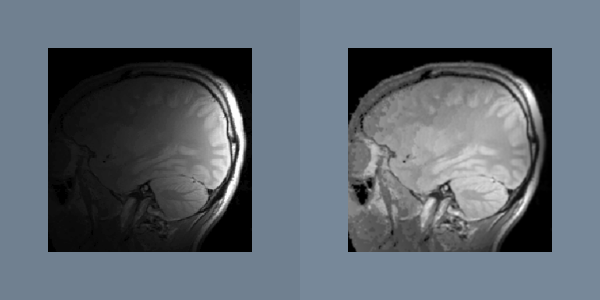
\includegraphics[width=0.96\linewidth]{Figure10-6a}
		\captionsetup{justification=centering}
		\caption*{(\href{https://lorensen.github.io/VTKExamples/site/Cxx/ImageProcessing/Attenuation/}{Attenuation.cxx} or \href{https://lorensen.github.io/VTKExamples/site/Python/ImageProcessing/Attenuation/}{Attenuation.py})} 
		\label{fig:Figure10-6a}
	\end{subfigure}
	\hfill
	\begin{subfigure}[h]{0.96\linewidth}
		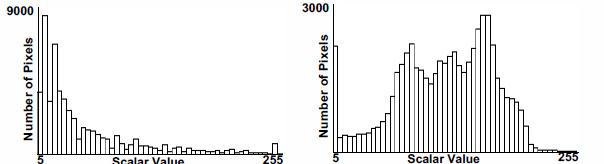
\includegraphics[width=0.96\linewidth]{Figure10-6b}
		\captionsetup{justification=centering}
		\caption*{}
		\label{fig:Figure10-6b}
	\end{subfigure}
	\caption{This MRI image illustrates attenuation that can occur due to sensor position. The artifact is removed by dividing by the attenuation profile determined manually. This histograms shows how the artifact hides information in the form of scalar value clusters.}\label{fig:Figure10-6}
\end{figure}

Another gradual change across an image is caused by sensor position\index{image artefact!sensor position}\index{sensor position!image artifact}. The amplitude of a measured signal usually attenuates as the source moves away from the sensor. An example of this attenuation artifact\index{attenuation artifact} is seen in surface--coil--MRI\index{Magnetic Resonance Imaging} images as shown in Figure \ref{fig:Figure10-6}. If the attenuation profile is known, then the artifact can be removed by dividing the original data with the profile. Since this artifact can be characterized by a small set of parameters like sensor position and range, it is possible to automatically determine the attenuation profile from the data. Like most artifacts, nonuniform attenuation tends to hide the information in an image. Given a function that measures the amount of information in an image, gradient descent and other search strategies can find the optimal attenuation parameters.
\index{image processing algorithms!low frequency artefacts|)}

\subsection{Image Enhancement}
\index{image enhancement|(}\index{image processing algorithms!image enhancement|(}

\begin{figure}[htb]
	\begin{subfigure}[h]{0.42\linewidth}
		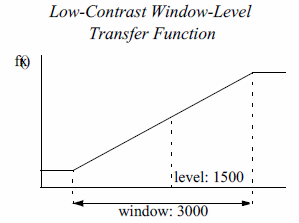
\includegraphics[width=0.96\linewidth]{Figure10-7a}
		\captionsetup{justification=centering}
		\caption*{}
		\label{fig:Figure10-7a}
	\end{subfigure}
	\hfill
	\begin{subfigure}[h]{0.42\linewidth}
		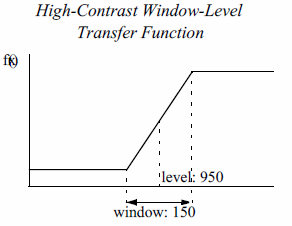
\includegraphics[width=0.96\linewidth]{Figure10-7b}
		\captionsetup{justification=centering}
		\caption*{}
		\label{fig:Figure10-7b}
	\end{subfigure}
	\hfill
	\begin{subfigure}[h]{0.42\linewidth}
		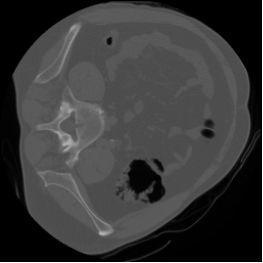
\includegraphics[width=0.96\linewidth]{Figure10-7c}
		\captionsetup{justification=centering}
		\caption*{}
		\label{fig:Figure10-7c}
	\end{subfigure}
	\hfill
	\begin{subfigure}[h]{0.42\linewidth}
		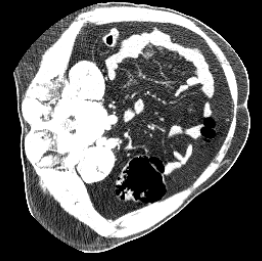
\includegraphics[width=0.96\linewidth]{Figure10-7d}
		\captionsetup{justification=centering}
		\caption*{}
		\label{fig:Figure10-7d}
	\end{subfigure}
	\hfill
	\begin{subfigure}[h]{0.42\linewidth}
		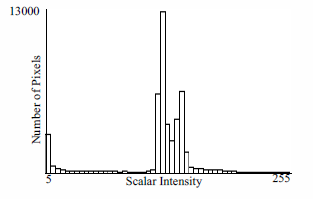
\includegraphics[width=0.96\linewidth]{Figure10-7e}
		\captionsetup{justification=centering}
		\caption*{}
		\label{fig:Figure10-7e}
	\end{subfigure}
	\hfill
	\begin{subfigure}[h]{0.42\linewidth}
		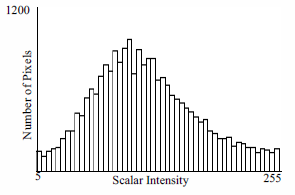
\includegraphics[width=0.96\linewidth]{Figure10-7f}
		\captionsetup{justification=centering}
		\caption*{}
		\label{fig:Figure10-7f}
	\end{subfigure}
	\caption{The top charts show two window-level transfer functions. The resulting images are displayed in the middle row. The bottom row shows image histograms of the images.}\label{fig:Figure10-7}
\end{figure}

Often datasets contain information or have dynamic range that cannot be completely displayed in a single image. X--Ray Computed Tomography\index{Computed Tomography} (CT) datasets, for example, can have 10 times the scalar resolution of the typical computer monitor capable of displaying 256 shades of gray. One method used for conveying information buried in the large dynamic range of these medical datasets is to allow a user to interactively set the color map with a window--level transfer function\index{image enhancement!window--level}. The user can then choose to display the range of data they find most important as shown in Figure \ref{fig:Figure10-7}. The slope of the transfer function determines the amount of contrast in the final image. Slopes greater than one increase contrast, and slopes less than one decrease contrast. All contrast and information is lost in the scalar ranges where the transfer function is constant and has zero slope.

The short fall of simple window--level\index{window--level} transfer functions are their limited shape. More general nonlinear transfer functions can be more appropriate for certain datasets. One example is the logarithmic transfer function, $f(x) = K \log ( 1 + x )$ , which can be used to display image power spectrums (Figure \ref{fig:Figure10-10}). Most of the pixels in the power spectrum represent high frequencies, and have small values. However the smaller population of low-frequency pixels often have large values. The logarithmic function has the largest slope near zero, and therefore leaves the most contrast for pixels with small values. However, when the constant K is chosen correctly, none of the large pixel values become completely saturated.

To take advantage of all the available display contrast, images should have a uniform distribution of intensities. For continuous images, this intensity distribution is called the probability density function\index{probability density function} (PDF\index{PDF|see {probability density function}}). For discretely--sampled images with discrete scalar values, the image histogram has the same information as the PDF (Figure \ref{fig:Figure10-7}). A histogram\index{histogram} breaks the scalar range of an image into discrete non-overlapping bins. Each bin has a pixel count that represents the number of pixels whose scalar value falls in that bin's range.

To achieve the goal of a uniform scalar histogram, transfer functions can be used to spread out clusters in the histogram and compress scalar ranges that are under-represented in the image. To maintain the general appearance of the image, the transfer function should be monotonically increasing so that the brightness relation is maintained. To spread out clusters in the histogram, the slope of the transfer function should be large where the scalar densities are the highest, and the slope should be small in empty regions of the histogram.

\begin{figure}[htb]
	\begin{subfigure}[h]{0.86\linewidth}
		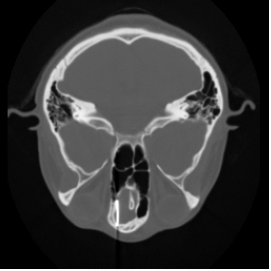
\includegraphics[width=0.48\linewidth]{Figure10-8a}
		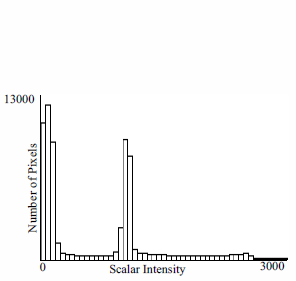
\includegraphics[width=0.48\linewidth]{Figure10-8b}
		\captionsetup{justification=centering}
		\caption*{Original image and its histogram}
		\label{fig:Figure10-8a}
	\end{subfigure}
	\hfill

	\begin{subfigure}[h]{0.48\linewidth}
		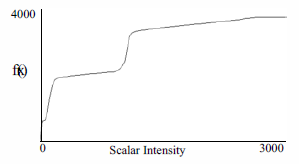
\includegraphics[width=0.96\linewidth]{Figure10-8c}
		\captionsetup{justification=centering}
		\caption*{Computer transfer function}
		\label{fig:Figure10-8c}
	\end{subfigure}

	\hfill
	\begin{subfigure}[h]{0.86\linewidth}
		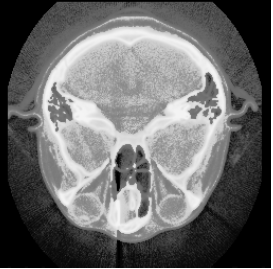
\includegraphics[width=0.48\linewidth]{Figure10-8d}
		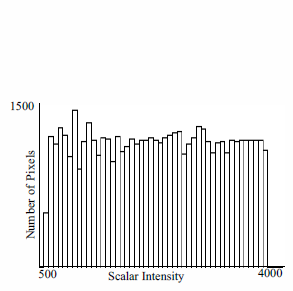
\includegraphics[width=0.48\linewidth]{Figure10-8e}
		\captionsetup{justification=centering}
		\caption*{Resulating image and its histogram}
		\label{fig:Figure10-8d}
	\end{subfigure}
	\caption{Histogram equalization automatically computes a transfer function that produces an image with a nearly constant scalar histogram.}\label{fig:Figure10-8}
\end{figure}

Histogram equalization\index{image enhancement!histogram equalization} is an algorithm that automatically generates a tailored transfer function to increase contrast in an image. For continuous images, the transfer function is simply the cumulative distribution function (CDF) which is defined as the integral of the PDF. By definition, the CDF function has a large slope where the PDF has the largest value, and therefore gives the greatest contrast to scalar ranges that occur most frequently in an image. The result of using the CDF as a transfer function is an image with an ideal constant scalar distribution. For discrete images and image histograms, a discrete version of the CDF function can be used. However, because of the discrete approximation, the resulting image is not guaranteed to have a constant histogram (Figure \ref{fig:Figure10-8}).

\begin{figure}[!htb]
	\centering
	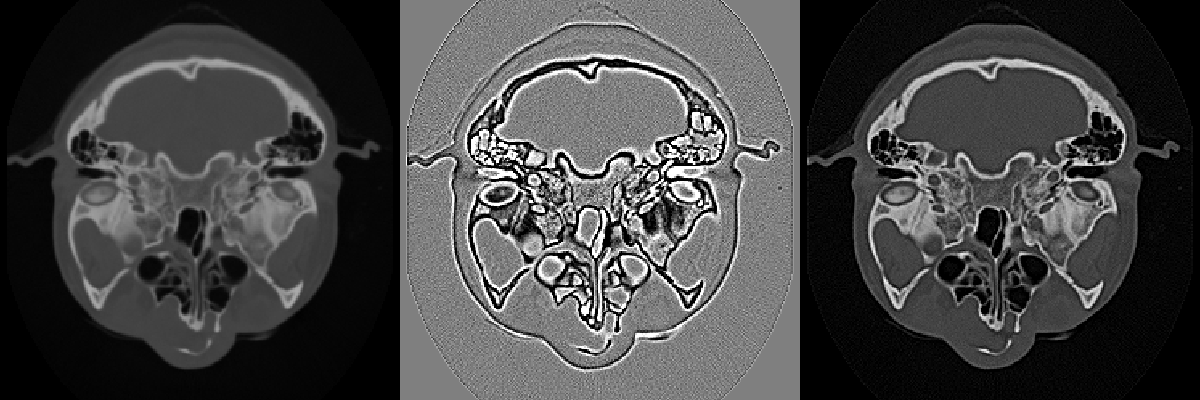
\includegraphics[width=0.98\textwidth]{Figure10-9}
	\caption{High-pass filters can extract and enhance edges in an image. Subtraction of the Laplacian (middle) from the original image (left) results in edge enhancement or a sharpening operation (right). (\href{https://lorensen.github.io/VTKExamples/site/Cxx/ImageProcessing/EnhanceEdges/}{EnhanceEdges.cxx} or \href{https://lorensen.github.io/VTKExamples/site/Python/ImageProcessing/EnhanceEdges/}{EnhanceEdges.py})}
	\label{fig:Figure10-9}
\end{figure}

High-pass filters can also be used to compress the range of an image. Since low frequencies account for much of the dynamic range of an image but carry little information, a high-pass filter can significantly decrease an image's scalar range and emphasize hidden details. The Laplacian filter\index{image enhancement!Laplacian filter}\index{Laplacian filter}, which is a second derivative operation, is one implementation of a high-pass filter. It eliminates constant and low frequencies leaving only high-frequency edges. The output of the Laplacian can be subtracted from the original image to produce edge enhancement or sharpening of an image (Figure \ref{fig:Figure10-9}).
\index{image enhancement|)}\index{image processing algorithms!image enhancement|)}

\subsection{Frequency Domain}
\index{frequency domain|(}\index{image processing algorithms!frequency domain|(}

\begin{figure}[!htb]
	\centering
	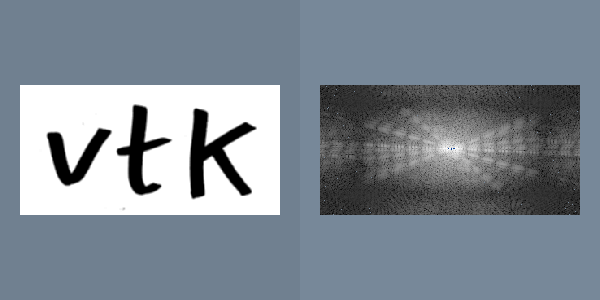
\includegraphics[width=0.98\textwidth]{Figure10-10}
	\caption{The discrete Fourier transform changes an image from the spatial domain into the frequency domain, where each pixel represents a sinusoidal function. This figure shows an image and its power spectrum displayed using a logarithmic transfer function. (\href{https://lorensen.github.io/VTKExamples/site/Cxx/ImageProcessing/VTKSpectrum/}{VTKSpectrum.cxx} or \href{https://lorensen.github.io/VTKExamples/site/Python/ImageProcessing/VTKSpectrum/}{VTKSpectrum.py}) The reverse Fourier Transform is: $F(u,v) = \dfrac{1}{M N}\mathlarger{\mathlarger{\sum}}_{x = 0}^{M - 1}\mathlarger{\mathlarger{\sum}}_{y = 0}^{N - 1}f(x,y)\exp \left[-j 2 \pi \left( \dfrac{x v}{M}  + \dfrac{v y}{N}\right) \right]$}
	\label{fig:Figure10-10}
\end{figure}

The Fourier transform\index{Fourier transform}\index{frequency domain!Fourier transform} belongs to a class of filters that fundamentally change the representation of an image without changing its information. The output of the Fourier transform is in the frequency domain. Each pixel is a complex number describing the contribution of a sinusoidal function to the original image. The magnitude of the pixel encodes the amplitude of the sinusoid, and the orientation of the complex pixel encodes the sinusoid's phase. Each pixel represents a sinusoid with different orientation and frequency. The reverse Fourier transform converts a frequency domain image back to the original spatial domain (Figure \ref{fig:Figure10-10}).

Low-pass and high-pass filtering become trivial in the frequency domain. A portion of the pixels are simply masked or attenuated. Figure \ref{fig:Figure10-10} shows a high pass Butterworth filter that attenuates the frequency domain image with the function $H$

\begin{equation}\label{eq:10.2}
H(u, v) = \dfrac{1}{1 + \left(\dfrac{C^2}{u^2 + v^2}\right)^n}
\end{equation}
\myequations{High pass Butterworth filter.}

\begin{figure}[htb]
    \begin{subfigure}[h]{0.48\linewidth}
        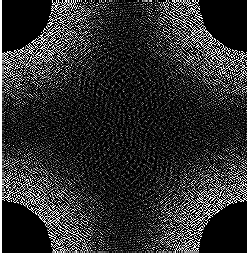
\includegraphics[width=0.96\linewidth]{Figure10-11a}
        \captionsetup{justification=centering}
        \caption*{Ideal High--Pass Filter $H(u,v) = \begin{dcases}
        1, & \text{if } \left( u^2 + v^2 < C^2 \right) \\
        0, & \text{otherwise}
        \end{dcases}$}
        \label{fig:Figure10-11a}
    \end{subfigure}
    \hfill
    \begin{subfigure}[h]{0.48\linewidth}
        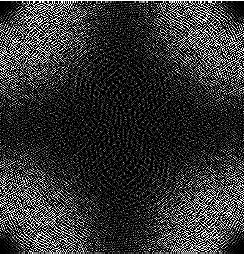
\includegraphics[width=0.96\linewidth]{Figure10-11b}
        \captionsetup{justification=centering}
        \caption*{Butterworth High--Pass Filter
        $H(u,v) = \dfrac{1} {1 + \left[ \dfrac{C^{2n}}{\left( u^2 + v ^2\right)^n} \right]} $}
        \label{fig:Figure10-11b}
    \end{subfigure}
    \hfill
    \begin{subfigure}[h]{0.96\linewidth}
        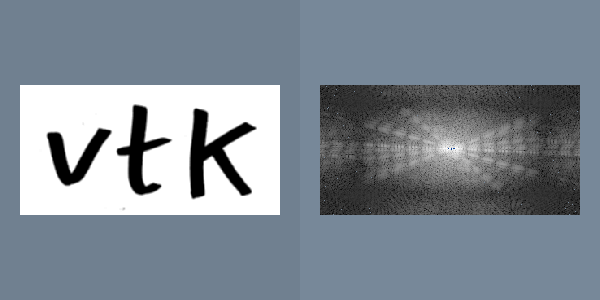
\includegraphics[width=0.96\linewidth]{Figure10-11c}
        \captionsetup{justification=centering}
        \caption*{See: (\href{https://lorensen.github.io/VTKExamples/site/Cxx/ImageProcessing/IdealHighPass/}{IdealHighPass.cxx} or \href{https://lorensen.github.io/VTKExamples/site/Python/ImageProcessing/IdealHighPass/}{IdealHighPass.py})}
        \label{fig:Figure10-11c}
    \end{subfigure}
    \caption{This figure shows two high-pass filters in the frequency domain. The Butterworth high-pass filter has a gradual attenuation that avoids ringing produced by the ideal high-pass filter with an abrupt transition.}\label{fig:Figure10-11}
\end{figure}

The gradual attenuation of the filter is important. The ideal high-pass filter, shown in the same figure, simply masks a set of pixels in the frequency domain. The abrupt transition causes a ringing effect in the spatial domain (as the figure illustrates).

Although any filter that operates in the frequency domain can also be implemented in the spatial domain, some operations are less computationally expensive and easier to implement in the frequency domain. To perform similar filtering of Figure \ref{fig:Figure10-11} in the spatial domain would require convolution with a large kernel and would be slow. In general, convolution with large kernels is more efficient when performed in the frequency domain. Multiplication,$\alpha \beta$, in the frequency domain, is equivalent to convolution,$a \star b$ , in the spatial domain (and vice versa). In these equations, $\alpha$ is the Fourier transform of $a$a, and $\beta$ is the Fourier transform of $b$.

In order to make frequency-domain processing feasible, it is first necessary to minimize the cost of transforming from the spatial to frequency domain and back. There exist fast algorithms that implement the Fourier transform and its inverse. First, the Fourier transform is decomposable, so a 2D transform can be implemented by first taking the 1D Fourier transform of all the rows, and then taking the Fourier transform of all the columns of an image. Second, the complexity of one-dimensional Fourier transforms can be reduced with an algorithm called the fast Fourier transform (FFT)\index{fast Fourier transform}\index{frequency domain!fast Fourier transform}. It works by recursively factoring the number samples, $N$, into its prime components. If $N$ is prime and not factorable, then the transform is completed in one step that is order $O(N^2)$ complexity. If $N$ is divisible by two, the array of numbers is divided into two parts that are transformed separately and then combined. If $N$ is a power of two, then the algorithm executes in order $O(N \log N)$ time.

For this reason, it is more efficient to process images with sizes that are powers of two (e.g., $512 \times 512$) than other sized images. For non-power of two images it may be faster to pad the image to a size that is a power of two size before processing.

An important point about the discrete Fourier transform is that it treats the image as a periodic function. This means the pixels on the right border are adjacent to pixels on the left border. Since there is usually no physical relationship between these pixels, the artificial horizontal and vertical edges can distort the frequency spectrum and subsequent processing. To reduce these artifacts, the original image can be multiplied by a window function that becomes zero at the borders. Another approach removes these artificial edges by smoothing only along the borders.

\begin{figure}[!htb]
	\centering
	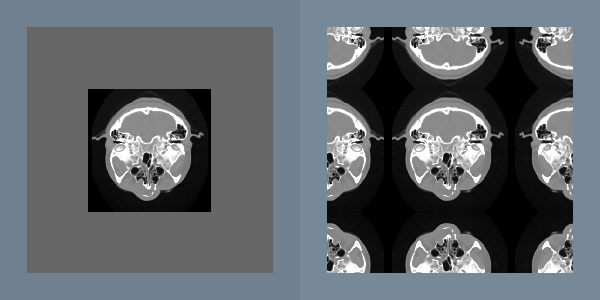
\includegraphics[width=0.98\textwidth]{Figure10-12}
	\caption{Convolution in frequency space treats the image as a periodic function. A large kernel can pick up features from both sides of the image. The left image has been padded with zeros to eliminate wraparound during convolution. On the right, mirror padding has been used to remove artificial edges introduced by borders. (\href{https://lorensen.github.io/VTKExamples/site/Cxx/ImageProcessing/Pad/}{Pad.cxx} or \href{https://lorensen.github.io/VTKExamples/site/Python/ImageProcessing/Pad/}{Pad.py})}
	\label{fig:Figure10-12}
\end{figure}


In both of these approaches, a portion of the original image is lost, so only the central portion of an image can be processed. If this is unacceptable, another solution is to double the dimensions of the original image with a mirror-padding filter. The intermediate image is periodic and continuous (Figure \ref{fig:Figure10-12}).
\index{frequency domain|)}\index{image processing algorithms!frequency domain|)}

\subsection {Image Segmentation}
\index{image processing algorithms!segmentation|(}\index{image segmentation|(}\index{segmentation|(}

Segmentation is the process of classifying pixels in an image or volume. It can be one of the most difficult tasks in the visualization process. One form of segmentation takes an image as input, and outputs a map that contains a classification for each pixel. The output of such a segmentation filter usually has binary or discrete values for each pixel; however, it is also possible to output a fuzzy classification where the pixel's scalar value represents a measure of confidence in the classification.

A simple example of a one-parameter segmentation is a threshold filter\index{image segmentation!threshold filter}\index{threshold filter} used to mark bone in a CT dataset. Since bone has the largest scalar value, it is easy to select a threshold that separates bone from the rest of the image.

\begin{figure}[htb]
    \begin{subfigure}[h]{0.16\linewidth}
        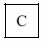
\includegraphics[width=0.96\linewidth]{Figure10-13a}
        \captionsetup{justification=centering}
        \caption*{Correlation Kernel}
        \label{fig:Figure10-13a}
    \end{subfigure}
    \hfill

    \hfill
    \begin{subfigure}[h]{0.48\linewidth}
        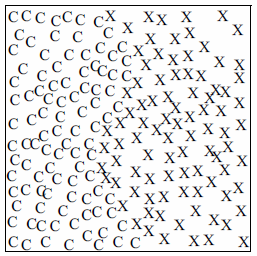
\includegraphics[width=0.96\linewidth]{Figure10-13b}
        \captionsetup{justification=centering}
        \caption*{Original Image}
        \label{fig:Figure10-13b}
    \end{subfigure}
    \hfill    
    \begin{subfigure}[h]{0.48\linewidth}
        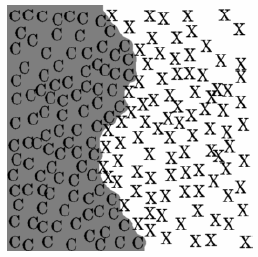
\includegraphics[width=0.96\linewidth]{Figure10-13c}
        \captionsetup{justification=centering}
        \caption*{Segmentation with Correlation}     
        \label{fig:Figure10-13c}
    \end{subfigure}
    \caption{A pipeline containing correlation, thresholding, dilation, and erosion is used here to segment a region composed of ``C''s. The left image shows the original image. The right image shows the segmented region superimposed on the original image.}\label{fig:Figure10-13}
\end{figure}

For other tissues and other imaging modalities, segmentation is usually more difficult. Noise in the image and overlapping scalar values of tissues can decrease the effectiveness of simple threshold segmentation. By using two parameters, the threshold can segment pixels with a range of scalar values. The extra parameter allows more control over the resulting segmentation, but also doubles the complexity of selecting the parameters.

Images can be preprocessed to segment images based on more complex features such as textures. Sometimes textures in tissues add information useful for segmentation. Texture sensitive filters like Laplacian and gradient magnitude can discriminate between different textures. Additional filters that can be used for texture segmentation are the range, variance, and correlation filters. The range filter simply reports the difference between the maximum and minimum values in a neighborhood around each pixel, and the variance filter computes the variance of the neighborhood pixels relative to the center pixel.

Figure \ref{fig:Figure10-13} shows an example of how a correlation filter\index{correlation filter}\index{image segmentation!correlation filter} can be used for segmentation. A correlation filter is similar to convolution. The kernel is shifted across the image, and for each location the dot product between the image and the kernel gives a measure of correlation between the two. The output of the correlation filter is large everywhere the pattern occurs in the image, but small at other locations. Because the resulting map is sparse, additional postprocessing is required to find a uniform, segmented region. In this example, dilation followed by erosion was used to close the gaps between the patterns. (Dilations and erosion are discussed in the next section.)
\index{image processing algorithms!segmentation|)}\index{image segmentation|)}\index{segmentation|)}

\subsection{Postprocessing}
\index{image processing algorithms!postprocessing|(}\index{postprocessing|(}

Although preprocessing can do a lot to improve segmentation results, postprocessing can also be useful. Morphological filters\index{morphological filter}\index{postprocessing!morphological filter}, which operate on binary or discrete images, can be useful for manipulating the shape of the segmented regions. In this brief discussion we will only consider operations that use circular footprints, even though these morphological filters can be defined much more generally. Erosion\index{erosion} is implemented by removing pixels within a specified distance of a border. For each pixel not in the segmented region, all the neighbors in a circular region around the pixels are turned off. This erosion filter shrinks the segmented region and small isolated regions disappear.

\begin{figure}[!htb]
	\centering
	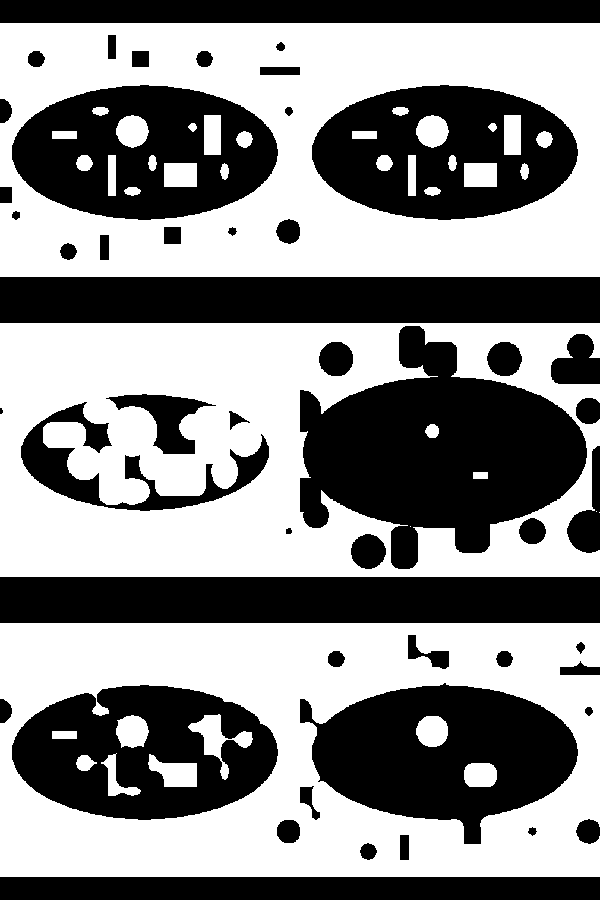
\includegraphics[width=0.63\linewidth]{Figure10-14}
	\caption{This figure demonstrates various binary filters that can alter the shape of segmented regions. From left to right: Original Image; Connectivity; Erosion; Dilation; Opening; Closing. (\href{https://lorensen.github.io/VTKExamples/site/Cxx/ImageProcessing/MorphologyComparison/}{MorphologyComparison.cxx} or \href{https://lorensen.github.io/VTKExamples/site/Python/ImageProcessing/MorphologyComparison/}{MorphologyComparison.py})}
	\label{fig:Figure10-14}
\end{figure}

The opposite of erosion is dilation\index{dilation}. This filter grows the area of segmented regions. Small holes in the segmented region are completely closed. Any pixel not in the segmented region but near the region is turned on. Dilation and erosion are dual filters with nearly identical implementations. Dilating the ``on'' pixels is equivalent to eroding ``off'' pixels in a binary image (see Figure \ref{fig:Figure10-14}).

Closing\index{closing} is the serial application of first dilation and then erosion. When an image is dilated small holes in the map disappear. However, dilation alone also grows the boundaries of the segmented regions. When dilation is followed by erosion in a closing operation, small holes are removed; however, the boundary of the segmented regions remain in the same general location. Opening\index{opening} is the dual of closing. Opening removes small islands of pixels. It is implemented with an initial erosion, followed by a dilation.

Connectivity\index{connectivity!in image processing}\index{postprocessing!connectivity} filters can also remove small regions without affecting the remaining boundaries of segmented regions. This set of filters separate the segmented pixels into equivalence classes based on a neighbor relation. Two pixels belong to the same class if they are touching. There are two common neighbor relations in two--dimensional images: four connectivity considers pixels neighbors if they are edge neighbors, and eight connectivity considers pixels neighbors if pixels share any vertex.

After the pixels have been assigned an equivalence class, various methods are used to determine which groups of pixels will pass through the filter, and which classes will be eliminated. The island--removal filter\index{island removal filter}\index{postprocessing!island removal filter} is a connectivity filter that removes groups that have too few pixels. Seed connectivity allows the user to explicitly specify which groups will pass through the filter. The user or application specifies a set of seeds. Any group that includes a seed makes it through the filter. Groups that do not contain seeds are removed. This filter is similar to the seed--connectivity filter; however, the seeds are supplied in a second image. First the intersection between the segmented image and the seed image is taken. Each remaining pixel is then added to a set of seeds.
\index{image processing algorithms!postprocessing|)}\index{postprocessing|)}

\subsection{Multispectral Segmentation}
\index{image processing algorithms!multi--spectral segmentation|(}\index{multi--spectral segmentation|(}\index{segmentation!multi--spectral|(}

From everyday experience we know that it is easier to see structure and information in color images than in gray--scale images. This is because each pixel contains more information in the red, blue, and green components than a single component gray-scale pixel. One way to segment multispectral images is to separate the components and threshold them individually and then combine the resulting binary images with logic filters. This allows selection of rectangular patched areas in the color/ component space of the pixels.

By using multiple thresholds combined with multiple levels of logic filters, it is possible to specify arbitrary areas in the component's space for segmentation. However, it can be easier and more efficient to transform the components into a different coordinate system before the threshold operation. The simplest example of this is to threshold a projection of the components. This is equivalent to a threshold after performing a dot product between the components of a pixel and a constant-direction vector. This divides the component space into two areas separated by a hyperplane.

Another example of a coordinate transformation is conversion from red, green, blue (RGB) color component to hue, saturation, value (HSV) representation (see ``Color'' on page \pageref{sec:color}). Segmentation of images based on hue and color saturation is difficult in RGB space, but trivial in HSV space.

Color is not the only multispectral information that can be used for segmentation. It is possible to take advantage of multispectral segmentation even if the original dataset has only one component. Additional images can be created from spatial information of the images using spatial filters. These multiple images can then be combined into one multicomponent image, then multicomponent segmentation can proceed.

Typically, the number of free parameters in a filter is directly correlated to the dimensionality of the pixels; and although additional parameters make a filter more powerful, it also makes it more difficult to find an appropriate set of parameter values. There are supervised and unsupervised algorithms that can be used to automatically select the best set of segmentation parameters, but discussion of these is outside the scope of this book.
\index{image processing algorithms!multi--spectral segmentation|)}\index{multi--spectral segmentation|)}
\index{algorithms!image processing|)}\index{image processing algorithms|)}\index{segmentation!multi--spectral|)}

\section{Putting It All Together}
\label{sec:chap10.putting_it_all_together}

We suggest that you review the code accompanying the images in this chapter to see how to use the VTK imaging pipeline. In this section we will explain some of the implementation details of image data. We will also show how to mix the imaging and visualization pipelines, and how to use imaging filters to perform regression testing.

\subsection{Data Representation}

In the imaging pipeline, the class for representing and manipulating data is vtkImageData see ``Types of Datasets'' on page \pageref{sec:types_of_datasets}). In addition, the data extent (topological extent specification) plays a vital role in controlling how images are processed.

vtkImageData\index{vtkImageData!and vtkDataArray} actually represents the image data. Internally, it refers to an instance of vtkDataArray. Therefore, its native representation data type may be any one of unsigned char, char, unsigned short, short, int, float, or any concrete type of vtkDataArray\index{vtkDataArray!and vtkImageData}. Please remember that vtkImageData can represent 1D, 2D (image), and 3D (volume) data.

There are three types of data extents\index{data extent} in the imaging pipeline. In general, any rectangular piece of image data can be described by the extent six-vector $(imin,imax, jmin,jmax, kmin,kmax)$. The WholeExtent refers to the original data size of an image and is derived from the image dimensions. The UpdateExtent is the extent that is processed by a particular filter during execution.

Extents are used to manage the streaming of data through the visualization pipeline, as well as to coordinate the multi-threaded parallel processing that the imaging pipeline uses throughout. By controlling the extents, it is possible to greatly reduce the amount of memory used by the pipeline. For more information, see The \emph{VTK User's Guide} sold by Kitware.

In the VTK imaging pipeline, point attribute data is represented differently than in the visualization pipeline. In the imaging pipeline point attribute data is represented as n components per data point. Typically n is one for gray-scale data, or three for color data but, in general, can be any positive number.

\subsection{Create an Image}
\index{image representation!implementation|(}

This example demonstrates how to directly create an image using C++ code. Typically, you will use an image reader or procedurally create an image from a source object. The example shown here creates an vtkImageData and then fills it with an image of interfering sinusoidal grids

\begin{equation}\label{eq:10.3}
F(x, y) = \sin\left(\frac{x}{10}\right) + \sin\left(\dfrac{y}{10}\right)
\end{equation}
\myequations{Sinusoidal grid.}

\begin{figure}[htb]
    \centering
	\begin{subfigure}[h]{0.48\linewidth}
		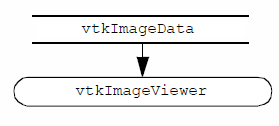
\includegraphics[width=0.96\linewidth]{Figure10-15a}
		\captionsetup{justification=centering}
		\caption*{}
		\label{fig:Figure10-15a}
	\end{subfigure}
	\hfill
	\begin{subfigure}[h]{0.48\linewidth}
		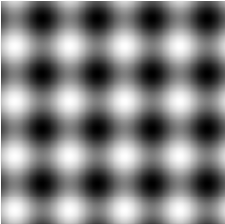
\includegraphics[width=0.96\linewidth]{Figure10-15b}
		\captionsetup{justification=centering}
		\caption*{}
        \label{fig:Figure10-15b}
	\end{subfigure}
	\hfill
	\begin{subfigure}[h]{0.96\linewidth}
       \begin{lstlisting}[language=C++,  caption={}, numbers=none, frame=none, escapechar=\$]
        int x, y;
        vtkImageData *image;
        
        image = vtkImageData$\index{vtkImageData!example}$::New();
          image->SetDimensions(256, 256, 1);
          image->SetScalarTypeToFloat();
          image->AllocateScalars();
        
        float *ptr = static_cast<float*>(image->GetScalarPointer());
        for (y = 0; y < 256; ++y)
          {
          for (x = 0; x < 256; ++x)
            {
            *ptr++ = 10.0 * sin(0.1 * x) * sin(0.1 * y);
            }
          }
        vtkImageViewer$\index{tkImageViewer!example}$ *viewer = vtkImageViewer::New();
          viewer->SetInput(image);
          viewer->SetColorWindow(20.0);
          viewer->SetColorLevel(0.0);
          viewer->Render();
        \end{lstlisting}
        \label{fig:Figure10-15d}
	\end{subfigure}
	\caption{Creating an image of two interfering sinusoidal gratings in an image dataset. The resulting image has dimensions $256^2$.}\label{fig:Figure10-15}
\end{figure}

Note that direct pointer access is used to fill the image. The AllocateScalars() method allocates enough memory for the dimensions provided.
\index{image representation!implementation|)}

\subsection{Gradient Magnitude}
\index{gradient magnitude!example|(}

\begin{figure}[htb]
    \centering
	\begin{subfigure}[h]{0.38\linewidth}
		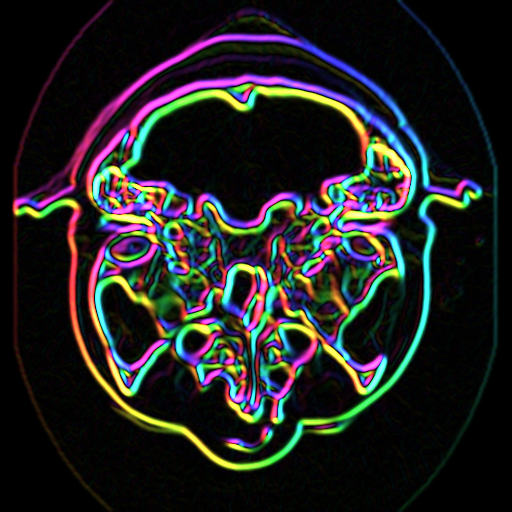
\includegraphics[width=0.96\linewidth]{Figure10-16a}
		\captionsetup{justification=centering}
		\caption*{See: (\href{https://lorensen.github.io/VTKExamples/site/Cxx/ImageProcessing/MorphologyComparison/}{MorphologyComparison.cxx} or \href{https://lorensen.github.io/VTKExamples/site/Python/ImageProcessing/MorphologyComparison/}{MorphologyComparison.py})}
		\label{fig:Figure10-16a}
	\end{subfigure}
	\hfill
	\begin{subfigure}[h]{0.38\linewidth}
		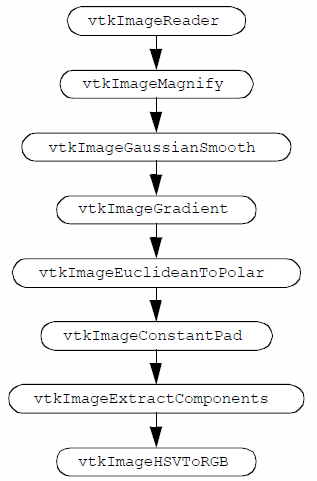
\includegraphics[width=0.96\linewidth]{Figure10-16b}
		\captionsetup{justification=centering}
		\caption*{}
        \label{fig:Figure10-16b}
	\end{subfigure}
	\hfill
	\begin{subfigure}[h]{0.78\linewidth}
       \begin{lstlisting}[language=TCL,  caption={}, numbers=none, frame=none, escapechar=\%]
        vtkImageGradient%\index{vtkImageGradient!example}% gradient
          gradient SetInputConnection [smooth GetOutputPort]
          gradient SetDimensionality 2
        
        vtkImageEuclideanToPolar%\index{vtkImageEuclideanToPolar!example}% polar
          polar SetInputConnection [gradient GetOutputPort]
          polar SetThetaMaximum 255
        
        vtkImageConstantPad%\index{vtkImageConstantPad}% pad
          pad SetInputConnection [polar GetOutputPort]
          pad SetOutputNumberOfScalarComponents 3
          pad SetConstant 200
        
        # permute components so saturation will be constant
        vtkImageExtractComponents permute
          permute SetInputConnection [pad GetOutputPort]
          permute SetComponents 0 2 1
          
        vtkImageHSVToRGB%\index{vtkImageHSVToRGB!example}% rgb
          rgb SetInputConnection [permute GetOutputPort]
          rgb SetMaximum 255
          \end{lstlisting}
        \label{fig:Figure10-16d}
	\end{subfigure}
	\caption{An imaging pipeline to visualize gradient information. The gradient direction is mapped into color hue value while the gradient magnitude is mapped into the color saturation.}\label{fig:Figure10-16}
\end{figure}

In this example we demonstrate a lengthy imaging pipeline. The basic purpose of the pipeline is to visualize information about the image gradient. The gradient direction and magnitude are mapped into the hue and saturation components of the color HSV space, respectively. The pipeline, resulting image, and a portion of the code are shown in Figure \ref{fig:Figure10-16}.

The pipeline demonstrates some interesting tricks. The first three filters read CT data of the human head (i.e., using vtkImageReader\index{vtkImageReader!example}), magnify the image by a factor of four (vtkImageMagnify\index{vtkImageMagnify!example}), and then smooth the data (since magnification uses linear interpolation, introducing some sharp edges). The next filter actually computes the 2D gradient (vtkImageGradient), placing the x-y gradient components into its output.

The next series of filters is where the fun begins. First, the data is converted to polar coordinates (vtkImageEuclideanToPolar\index{vtkImageEuclideanToPolar!example}). We use this filter because we want to operate in color HSV space (see ``Color'' on page \pageref{sec:color}). The image magnitude is to be mapped into saturation value, while the gradient direction is mapped into hue value (remember hue is represented as an angle on the HSV color wheel). The filter vtkImageConstantPad\index{vtkImageConstantPad!example} is used to add a third component to the data, since the gradient filter only generated two components, and we need three components to represent color. The vtkImageExtractComponents\index{vtkImageExtractComponents!example} is used to rearrange the components into HSV order. Finally, the data is converted back into RGB color space with vtkImageHSVToRGB\index{vtkImageHSVToRGB!example}. (This is necessary because the image viewer expects RGB values.)
\index{gradient magnitude!example|)}

\subsection{Image Warping}
\index{image warping!example|(}

\begin{figure}[htb]
    \centering
	\begin{subfigure}[h]{0.48\linewidth}
		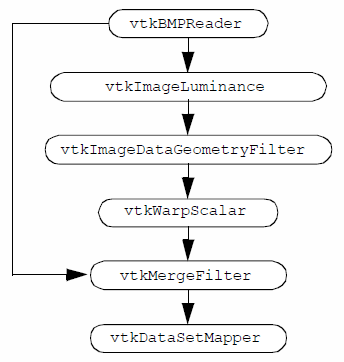
\includegraphics[width=0.96\linewidth]{Figure10-17a}
		\captionsetup{justification=centering}
		\caption*{}
		\label{fig:Figure10-17a}
	\end{subfigure}
	\hfill
	\begin{subfigure}[h]{0.48\linewidth}
		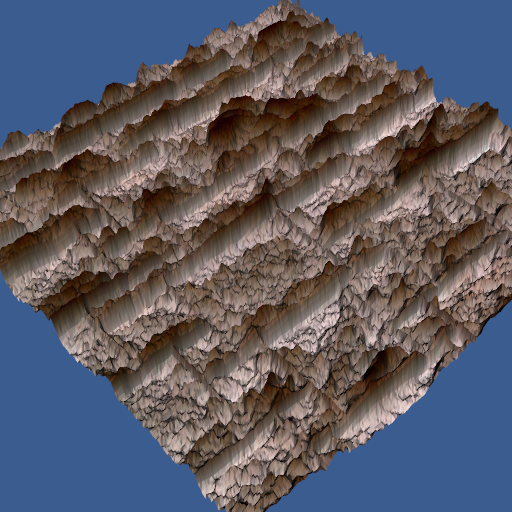
\includegraphics[width=0.96\linewidth]{Figure10-17b}
		\captionsetup{justification=centering}
		\caption*{See: (\href{https://lorensen.github.io/VTKExamples/site/Cxx/Images/ImageWarp/}{ImageWarp.cxx} or \href{https://lorensen.github.io/VTKExamples/site/Python/Images/ImageWarp/}{ImageWarp.py})}
        \label{fig:Figure10-17b}
	\end{subfigure}
	\hfill
	\begin{subfigure}[h]{0.96\linewidth}
       \begin{lstlisting}[language=TCL,  caption={}, numbers=none, frame=none, escapechar=\%]
        vtkBMPReader reader
          reader SetFileName $VTK_DATA_ROOT/Data/masonry.bmp
        vtkImageLuminance%\index{vtkImageLuminance!example}% luminance
          luminance SetInputConnection [reader GetOutputPort]
        vtkImageDataGeometryFilter%\index{vtkImageDataGeometryFilter!example}% geometry
          geometry SetInputConnection [luminance GetOutputPort]
        vtkWarpScalar%\index{vtkWarpScalar!example}% warp
          warp SetInputConnection [geometry GetOutputPort]
          warp SetScaleFactor -0.1
          
        vtkMergeFilter merge
          merge SetGeometryConnection [warp GetOutputPort]
          merge SetScalarsConnection [reader GetOutputPort]
        vtkDataSetMapper mapper
          mapper SetInputConnection [merge GetOutputPort]
          mapper SetScalarRange 0 255
          mapper ImmediateModeRenderingOff
        \end{lstlisting}
        \label{fig:Figure10-17d}
	\end{subfigure}
	\caption{Combining the imaging and visualization pipelines to deform an image in the z-direction. The vtkMergeFilter is used to combine the warped surface with the original color data.}\label{fig:Figure10-17}
\end{figure}

In this example we combine the imaging and visualization pipelines. Imaging filters are used to read in an image (vtkBMPReader\index{vtkBMPReader}) and then convert it to grayscale (vtkImageLuminance\index{vtkImageLuminance!example}). The data, which is a image data dataset, is then passed down the visualization pipeline as polygons using vtkImageDataGeometryFilter\index{vtkImageDataGeometryFilter!example}. Next we warp the data in the direction perpendicular to the image plane using the visualization filter vtkWarpScalar\index{vtkWarpScalar}. The vtkMergeFilter\index{vtkMergeFilter} is used to combine the warped geometry (now vtkPolyData) with the original image data from the reader. (Note that in this example the vtkMergeFilter takes two inputs.) The pipeline, example output, and sample code are shown in Figure \ref{fig:Figure10-17}.
\index{image warping!example|)}

\subsection{Regression Testing}
\index{regression testing!example|(}

In our work with VTK, we often need to perform software testing. The testing may be necessary because we’ve added new classes or features to the system, modified old code, or are simply testing a graphics library or new piece of hardware. We use a powerful testing procedure based on processing the output of the system, which is typically an image. We refer to the testing process as regression testing.

\begin{figure}[htb]
    \centering
	\begin{subfigure}[h]{0.32\linewidth}
		
\includegraphics[width=0.96\linewidth]{Figure10-18a}
		\captionsetup{justification=centering}
		\caption*{Valid}
		\label{fig:Figure10-18a}
	\end{subfigure}
	\hfill
	\begin{subfigure}[h]{0.32\linewidth}
		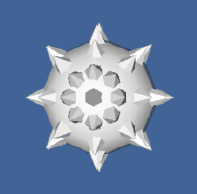
\includegraphics[width=0.96\linewidth]{Figure10-18b}
		\captionsetup{justification=centering}
		\caption*{Test}
        \label{fig:Figure10-18b}
	\end{subfigure}
	\hfill
	\begin{subfigure}[h]{0.32\linewidth}
		
\includegraphics[width=0.96\linewidth]{Figure10-18c}
		\captionsetup{justification=centering}
		\caption*{Difference}
        \label{fig:Figure10-18c}
	\end{subfigure}
	\hfill
	\begin{subfigure}[h]{0.96\linewidth}
       \begin{lstlisting}[language=TCL,  caption={}, numbers=none, frame=none]
        vtkRendererSource renSrc
          renSrc WholeWindowOn
          renSrc SetInput ren1
        vtkPNGReader pnm
          pnm SetFileName 'valid/$afile.png'
        vtkImageDifference imgDiff
          imgDiff SetInputConnection 0 [renSrc GetOutputPort]
          imgDiff SetInputConnection 1 [pnm GetOutputPort]
          imgDiff Update
        if {[imgDiff GetThresholdedError] < 10.0} {
          puts "Passed Test for $afile"
        } else {
          puts "Failed Test for $afile with an error \
            of [imgDiff GetThresholdedError]"
          vtkPNGWriter pnmw
            pnmw SetInputConnection [imgDiff GetOutputPort]
            pnmw SetFileName "$afile.error.png"
            pnmw Write
          vtkPNGWriter pnmw2
            pnmw2 SetInputConnection [renSrc GetOutputPort]
            pnmw2 SetFileName "$afile.test.png"
            pnmw2 Write
        }
        \end{lstlisting}
        \label{fig:Figure10-18d}
	\end{subfigure}
	\caption{Software regression testing using image processing. A test image is taken from the renderer and compared with a valid image stored on disk. (a) shows the valid image. (b) shows the test image (artificially modified by slight camera rotation). (c) shows the image difference. The code fragment above is extracted from the regression testing procedure.}\label{fig:Figure10-18}
\end{figure}

Regression testing is based on the following procedure. A test program (typically a Tcl/Tk script) is written that exercises a portion of the code. In our example, we will assume that we are testing a feature of implicit modelling. The output of the script is an image with a fixed view, as shown in Figure \ref{fig:Figure10-18}(a). To perform the test, we compare the output of the test program with a previously stored image, or ``valid'' image (Figure \ref{fig:Figure10-18}(b)). The valid image was generated when we initially created the object or objects to be tested, and is assumed to be the correct output. Then, we use a the filter vtkImageDifference\index{vtkImageDifference!example} to compare the test image with the valid image. This filter takes into account dithering and anti-aliasing effects, and creates an output image representing the difference between the test image and valid image (Figure \ref{fig:Figure10-18}(c)). It also reports the difference in the images in terms of a pixel count. To determine whether the test is passed, we compare the pixel count with a threshold value (for example, 10 pixels).

Our regression testing procedure cannot test the original implementation of an object or objects. The developer must verify that the valid image is indeed correct. However, the process is invaluable for finding and correcting problems due to incremental code changes (e.g., bug fixes, enhancements, etc.) Furthermore, the test can be run as a batch process, with a simple pass/fail output, and an image to show the differences.
\index{regression testing!example|)}
\index{image processing|)}

\section{Chapter Summary}

Image processing can be used to improve 3D visualizations of structured point datasets (images and volumes). Important techniques include smoothing, filtering, morphological operators such as erosion and dilation, and segmentation.

Because of the regular topology and geometry of images, it is possible to design caching and streaming pipelines to reduce memory requirements. In the \emph{Visualization Toolkit}, the imaging pipeline is integrated with the visualization pipeline. This capability enables the creation of applications that combine computer graphics, imaging, and visualization.

\section{Bibliographic Notes}

Many books are available describing imaging algorithms. Several are listed below including \cite{Gonzalez92} and \cite{Russ95}. The texts \cite{Pavlidis82} and \cite{Wolberg90} are imaging books with somewhat of a computer graphics and/or visualization slant. The text \cite{Robb95} is an outstanding reference for medical imaging and visualization.

If image processing, segmentation, and/or registration are important to you, we highly recommend the Insight Segmentation and Registration Toolkit (ITK). Like VTK, ITK is open source and includes extensive documentation resources and examples. Visit \href{https://itk.org/}{ITK} for more information. Also, \cite{Ibanez03} is a good reference.

Technical references describing VTK's unique streaming visualization pipeline are available \cite{Law99} \cite{Martin01}. Using this approach, data sizes of approximately a petabyte in size have been processed.


\printbibliography

\section{Exercises}

\begin{figure}[!htb]
	\centering
	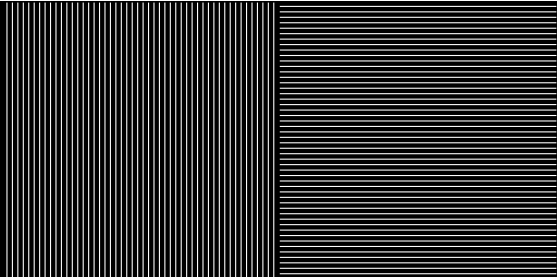
\includegraphics[width=0.98\textwidth]{Figure10-19}
	\caption{Sample image for segmentation exercise.}
	\label{fig:Figure10-19}
\end{figure}

\begin{enumerate}

\item Create an image pipeline that will segment the area with vertical lines in Figure \ref{fig:Figure10-19}.

\item Decomposition can increase the speed of an operation.

    \begin{enumerate}

    \item Prove that 3D Gaussian smoothing can be decomposed into three 1D operations.

    \item Determine the complexity of the decomposed filter and the same filter implemented as a 3D convolution.

    \item Under what conditions can constant smoothing be decomposed into 1D operations?

    \end{enumerate}

\item Create an image pipeline that shows the spectrum of a Gaussian image. What effect does increasing or decreasing the standard deviation have on the spectrum?

\end{enumerate}
